\documentclass[a4paper]{easychair}
\usepackage[utf8]{inputenc}
\usepackage[T1]{fontenc}
\usepackage[french]{babel}
\usepackage{minted}
\usepackage{hyperref}
\usepackage{amsfonts}
\usepackage{multicol}
\usepackage{tikz}
\usetikzlibrary{arrows}
\usepackage{macros}

\title{Détection de définitions OCaml similaires \\
(ou comment ne plus voir double à dos de chameau)}

\author{Alexandre Moine et Yann Régis-Gianas}

\institute{Université de Paris}

\authorrunning{Moine et Régis-Gianas}
\titlerunning{Détection de définitions OCaml similaires}
\begin{document}

\maketitle

\begin{abstract}
L'absence de redondance est souvent un gage de qualité pour un code
source. En effet, lorsqu'un fragment de code est répété, ses
imperfections -- pour ne pas dire ses erreurs -- le sont elles-aussi.

Seulement, il arrive parfois que l'on constate de la redondance dans
un grand corpus de code, typiquement quand ce corpus a été construit
par des développeurs ne communiquant peu ou pas du tout entre
eux. Deux instances de cette situation nous intéressent
particulièrement : l'ensemble des codes sources des paquets {\Opam} et
l'ensemble des copies d'étudiants répondant tous aux mêmes questions
de programmation. Comment partitionner leurs définitions en fonction
de leur ``similarité''?

Dans cet article, nous proposons un outil de partitionnement
automatique d'un ensemble de définitions écrites en OCaml. Cet outil
s'appuie sur une fonction dédiée de prise d'empreintes des arbres de
syntaxe du langage intermédiaire {\LambdaCode} ainsi que sur un
algorithme de classification hiérarchique classique que nous avons
adapté à notre usage.

Cet outil prend la forme d'une bibliothèque nommée {\Asak} disponible
sur {\Opam}. Nous l'avons utilisée d'une part pour partitionner
automatiquement les réponses d'étudiants qui apprennent OCaml en
utilisant la plateforme {\LearnOCaml}, et d'autre part, pour détecter des
redondances sur l'ensemble des codes sources des paquets~{\Opam}
disponibles aujourd'hui. Nous évaluons les résultats obtenus et
formulons quelques limites de notre approche.

\end{abstract}

\section{Introduction}
%!TEX root = root.tex

``Ne vous répétez pas!'' est une injonction permanente qui plane au
dessus de tout programmeur cherchant à écrire un logiciel de qualité.
Ce principe vise une situation idéale où une connaissance donnée n'a
qu'une seule représentation dans le logiciel : si cette connaissance
est imparfaite -- et c'est souvent le cas -- on s'assure alors qu'elle
pourra être corrigée efficacement.

Il arrive parfois qu'un corpus de code source contienne des
redondances que les programmeurs n'ont pas pu ou pas voulu éviter. Par
exemple, certaines fonctions utilitaires absentes de la bibliothèque
standard sont ainsi réimplémentées à de multiples reprises par de
nombreux paquets logiciels. L'implémentation de ces fonctions
utilitaires répétées sont parfois identiques aux caractères près ;
parfois, elles sont seulement très proches (à quelques renommages près
ou plus généralement, à quelques réécritures ``bénignes''
près). Ainsi, si l'on utilise deux bibliothèques indépendantes pour
construire un logiciel donné, il y a une probabilité non nulle que
l'on retrouve dans l'exécutable final plusieurs implémentations
quasi-identiques de la même fonction. Ne serait-il pas plus
raisonnable d'introduire une bibliothèque commune offrant une unique
implémentation de ces fonctions répétées?

Il y a aussi des redondances dont les programmeurs n'ont pas conscience.
En effet, on peut parfaitement appliquer ``la tête dans le guidon''
des schémas de calcul généraux en les spécialisant à des arguments
particuliers, au cas par cas, sans réaliser les opportunités de
factorisation qui découleraient de l'introduction d'une fonction
d'ordre supérieur bien choisie. C'est seulement lorsque les
développeurs prennent un peu de recul qu'ils s'aperçoivent qu'une
factorisation du code source est possible. Ne serait-il pas plus
raisonnable d'alerter le programmeur à la minute même où il introduit
un fragment de code qui est fortement similaire à un autre fragment
préexistant, soit dans son propre code, soit dans une autre
bibliothèque?

Lorsqu'un corpus est formé de réponses d'étudiants à des questions
identiques de programmation, il y a fort à parier que plusieurs
étudiants répondront de façon similaire à une question donnée, soit
parce qu'ils ont trouvé une réponse ``naturelle'', soit parce qu'ils
ont commis des erreurs de raisonnement ou de conception classiques.
Pour l'enseignant face à plusieurs centaines de réponses, il n'est pas
toujours évident de réaliser quelles sont les classes
qui partitionnent pertinemment l'ensemble de ces réponses. Lui
apporter un tel partitionnement serait un outil précieux car il
lui permettrait de différencier sa pédagogie en fonction des
groupes de réponses fausses les plus courantes.

Pour répondre à ces trois cas d'usage, il faudrait tout d'abord que
l'on sache évaluer la ``similarité'' entre deux fragments de
code. Mais qu'entend-on exactement par similarité? Peut-on
formaliser cette notion et la réaliser calculatoirement?

Notons tout d'abord que nous avons utilisé le terme de similarité et
non d'équivalence. En effet, la notion d'équivalence (syntaxique,
définitionnelle ou observationnelle) est trop ``binaire'' pour notre
cadre : nous cherchons une mesure qui rapproche des calculs qui se
ressemblent même s'ils ne se comportent pas tout à fait de la même
façon calculatoirement. En d'autres termes, nous cherchons des
fragments de programme qui ont des structures syntaxiques proches et
qui s'appuient sur des ingrédients similaires plutôt que des fragments
de programme ne pouvant pas être distingués par des contextes
d'évaluation.

Ainsi, deux termes égaux syntaxiquement sont absolument similaires.
Deux termes qui diffèrent par un renommage sont très similaires sans
être syntaxiquement égaux. Deux analyses par motifs sont plus ou
moins similaires en fonction des cas d'analyse qu'elles traitent
de façon similaire. Par contre, les implémentations de deux
algorithmes de tri distincts sont en général dissimilaires
même si l'équivalence observationnelle ne permet pas de les
distinguer\footnote{Bien entendu, on suppose ici
un langage de programmation incapable d'observer finement
les exécutions des deux algorithmes.}.

La similarité semble donc être une notion très syntaxique mais qui
cherche paradoxalement à faire peu de cas de certains détails
d'écriture qui ne changent pas fondamentalement le programme que l'on
a écrit. De toute évidence, toutes les différences purement textuelles
(commentaires, indentations, ...) doivent être ignorées par une bonne
notion de similarité. Le renommage des variables liées est aussi un
exemple canonique de tels détails syntaxiques anodins. Plus
généralement, toute transformation locale et purement syntaxique,
i.e. toute élimination de sucre syntaxique, semble aussi rentrer dans
cette catégorie des ``détails syntaxiques''. Où s'arrêter dans ce
processus de simplification des termes? Devrait-on par exemple aller
jusqu'à comparer les codes machines obtenus par compilation des termes
sources? Cette démarche conduirait sans doute à un échec puisque le
jeu de la sélection d'instructions et des différentes optimisations
peut mener deux termes sources proches à des codes machines très différents
et fourmillant de nouveaux détails peu importants (pensez à la
diversité des instructions d'une architecture comme x86-64). Il faut
donc trouver le langage intermédiaire offrant un bon niveau
d'abstraction pour éliminer à la fois les détails syntaxiques
du langage source et les détails de bas-niveau de l'architecture cible.

La première contribution de cet article est de considérer que les
premières passes du compilateur {\OCaml}, celles menant de sa syntaxe
concrète au code {\LambdaCode}, éliminent la plupart des détails
syntaxiques des termes {\OCaml} pour ne garder que leurs ingrédients
calculatoires principaux. Nous analyserons les avantages
(sections~\ref{sec:partition} et \ref{sec:redundancy}) et les
limitations (section~\ref{sec:limitations}) de ce choix de conception.

Comme son nom l'indique, {\LambdaCode} est un $\lambda$-calcul
(légèrement étendu). Nous nous sommes donc moralement ramené au
problème de la construction d'une mesure de dissimilarité syntaxique
entre deux termes du $\lambda$-calcul. En utilisant une représentation
de De Bruijn et en effectuant quelques réductions inoffensives, on
gomme effectivement de cette façon certaines différences sans intérêt
entre deux termes {\OCaml}. Seulement, pour pouvoir comparer
rapidement des milliers de $\lambda-$termes deux-à-deux, on doit se
donner une représentation compacte des $\lambda$-termes. Nous
introduisons donc un prétraitement des $\lambda$-termes pour calculer leurs \textit{empreintes}
respectives : l'empreinte d'un $\lambda$-terme est un ensemble
d'entiers qui caractérisent ses aspects syntaxiques importants. C'est
une idée déjà présente dans la littérature mais nous la raffinons pour
l'appliquer sur des $\lambda$-termes.  La définition de ce
prétraitement sur des $\lambda$-termes est donc la seconde
contribution présentée par cet article.

À ce stade, on peut donc mesurer la dissimilarité entre chaque paire de termes d'un corpus. L'ensemble de ces mesures
constitue une grande quantité d'information peu structurée
difficilement exploitable directement, en tout cas pour nos cas
d'usage. Pour pallier à ce problème, nous proposons de partitionner hiérarchiquement
les termes en s'appuyant sur leur mesure de dissimilarité
(section~\ref{sec:clustering}). Encore une fois, notre contribution
consiste à raffiner un algorithme déjà présent dans la littérature, la
classification ascendante hiérarchique. Cette classification produit
des dendrogrammes, particulièrement adaptés à l'exploration des
classes de programmes issues de nos corpus.

Pour que notre travail soit réutilisable dans des situations
différentes de nos cas d'usage, nous avons développé une bibliothèque
nommée {\Asak}\footnote{Cette bibliothèque fait des partitions (de codes similaires), son nom est donc tiré de la musique: asak est un genre de chansons touareg.}.
Cette bibliothèque est librement disponible sous la forme d'un paquet {\Opam}.
Elle nous a permis d'introduire un système de classification automatique
des copies dans {\LearnOCaml} (section~\ref{sec:partition}). Elle nous a
aussi permis d'implémenter un outil de recherche de redondance dans
l'ensemble des paquets {\Opam} (section~\ref{sec:redundancy}). Ces outils
constituent la dernière contribution présentée par cet article.


\section{Vue d'ensemble de l'approche}
\label{sec:overview}
Dans cette section, nous décrivons le fonctionnement de notre outil
sur un corpus d'exemple et nous expliquons certains de nos choix de
conception par la même occasion.

\begin{figure}
\begin{multicols}{2}
\begin{ocaml}
(* Code 1 *)
let rec rev l = match l with
    [] -> []
  |t::q -> rev q@[t]

(* Code 2 *)
let rec rev l =
  match l with
  | [] -> []
  | a::t -> (rev t)@[a]

(* Code 3 *)
let rec rev l = match l with
    [] | [_] -> l
  | t::q -> rev q@[t];;
\end{ocaml}
\begin{ocaml}
(* Code 4 *)
let rev l=
  let rec rev_aux acc l=
    match l with
    |[]->acc
    |t::q->rev_aux (t::acc) q
  in rev_aux [] l

(* Code 5 *)
let rev l =
  match l with
    [] -> []
  |a::q -> let rec rev2 x y = match y with
        [] -> x
      |b::z -> rev2 (b::x) z in rev2 [] l

(* Code 6 *)
let rev l =
  List.fold_left (fun acc x -> x :: acc) [] l
\end{ocaml}
\end{multicols}
\label{fig:example:sources}
\caption{Un corpus jouet pour illustrer notre algorithme.}
\end{figure}


\paragraph{Que produit {\Asak}?}
{\Asak} compare entre elles les définitions globales d'un ensemble de
modules {\OCaml}. La figure~\ref{fig:example:sources} contient cinq
exemples de telles définitions {\OCaml}. Elles forment un corpus jouet
qui va nous servir à illustrer le fonctionnement d'{\Asak}.  Le
lecteur aura reconnu d'un coup d'{\oe}il la fonction classique qui
renvoie la liste mirroir d'une liste prise en argument et l'enseignant
aura reconnnu des réponses typiques d'étudiants apprenti-programmeurs
fonctionnels. Sur ce corpus, notre outil produit l'ensemble de
dendrogrammes de la figure~\ref{fig:toy-classes}.

\begin{figure}
\begin{center}
\begin{tikzpicture}[sloped, scale=0.5]
\node (a)  at (-6,0)   {1};
\node (b)  at (-5,0)   {2};
\node (ab) at (-5.5,1) {};
\node (c) at (-3,0) {3};
\node (abc) at (-4, 2) {};
\node (d) at (-2,0) {4};
\node (e) at (-1,0) {5};
\node (de) at (-1.5,2) {};
% \node (abcde) at (-3.5, 3) {};
\node (f) at (0,0) {6};
%\node (all) at (-1, 4) {};
%\node (root) at (-1,5) {};

\draw  (a) |- (ab.center);
\draw  (b) |- (ab.center);
\draw  (ab) |- (abc.center);
\draw  (c)  |- (abc.center);
%\draw  (abc) |- (abcde.center);
%\draw  (de)  |- (abcde.center);
\draw  (d)  |- (de.center);
\draw  (e)  |- (de.center);

%\draw  (abcde) |- (all.center);
%\draw  (f)     |- (all.center);

%\draw (all)      |- (root.center);

\draw[->,-triangle 60] (-7,0) -- node[above]{dissimilarité} (-7,6);
\end{tikzpicture}
\end{center}
\caption{Ensemble de dendrogrammes correspond à la classification du corpus jouet.}
\label{fig:toy-classes}
\end{figure}

Un dendrogramme est un arbre binaire dont les n{\oe}uds représentent
des classes d'individus. Les feuilles de ces dendrogrammes sont les
différentes versions de \texttt{rev}. Un dendrogramme fournit un
partitionnement hiérarchique d'un ensemble d'invididus: en le
parcourant d'une feuille vers sa racine, on découvre des classes
d'invididus de plus en plus dissimilaires à cette feuille ; en le
parcourant de sa racine vers ses feuilles, on découvre des séparations
successives en deux classes d'un ensemble d'individus maximisant la
dissimilarité entre les membres des deux classes. Dans la sortie
de notre outil, deux classes qui appartiennent à deux dendrogrammes
distincts sont absolument dissimilaires, i.e. elles n'ont rien en
commun.

Dans le cas de ce corpus, le regroupement des définitions~$1$ et~$2$
est très naturel puisque ces deux définitions sont équivalentes à
quelques détails purement textuels près : la présence du \iocaml{|},
d'un retour à la ligne et d'un renommage. La définition~$3$ est proche
de cette première classe: elle en diffère seulement à cause d'un cas
d'analyse supplémentaire. Le regroupement des définitions~$4$ et~$5$
est assez naturel puisqu'elles suivent la même (et bonne!) stratégie
qui consiste à accumuler le résultat dans l'argument d'une fonction
auxiliaire interne. Notons que ces deux définitions sont dissimilaires
même si elles utilisent les mêmes ``ingrédients'' : la définition~$5$
effectue une analyse par cas supplémentaire pour traiter le cas de la
liste vide de façon spécifique.
%% Les deux classes~$(1-2)-3$
%% et~$4-5$ partagent le fait d'être des définitions récursives procédant par
%% analyse de cas : ces individus sont clairement séparés de la définition~$6$
%% qui s'appuie sur une spécialisation de la fonction~\iocaml{List.fold_left}.

%% L'intérêt d'une classification hiérarchique est surtout visible sur de
%% grands corpus : les quelques classes les plus proches de la racine du
%% dendrogramme sont les principales classes de définitions similaires
%% -- celles qui partagent au moins un sous-terme -- et c'est
%% en observant chaque classe en profondeur que l'on raffine petit à
%% petit les différences entre ses membres.

\paragraph{Comment procède {\Asak}?}
Ce partitionnement semble assez naturel mais comment
notre outil l'a-t-il obtenu? Comme nous l'avons déjà écrit dans
l'introduction, le traitement de notre outil se décompose
essentiellement en trois étapes: (i) les programmes sources sont
normalisés pour ignorer les détails syntaxiques que nous jugeons
inessentiels ; (ii) on calcule une empreinte pour caractériser la
structure et les ingrédients principaux des programmes normalisés ;
(iii) on applique un algorithme de partitionnement hiérarchique qui
s'appuie sur les empreintes.

\paragraph{Comment les définitions sont-elles normalisées?}
L'analyse syntaxique est la solution canonique pour éliminer les
artefacts textuels et ne garder que la structure d'un code source.
Notre outil travaille donc sur des arbres de syntaxe abstraits.  On
pourrait opposer à ce choix de conception le fait que considérer le
texte des programmes permettrait de séparer des programmes dont les
arbres de syntaxe sont égaux. Cependant, un tel point de vue sépare
trop de programmes.

Une fois que l'on a décidé de travailler sur un langage d'arbres
distincts de la syntaxe concrète, il faut choisir ce nouveau langage.
On aurait pu choisir de traduire les termes sources vers un langage
conçu pour l'occasion mais ce serait beaucoup de travail. Il existe
heureusement un langage intermédiaire adéquat dans le
compilateur~{\OCaml}: le langage {\LambdaCode}. Nos expérimentations
nous portent à croire qu'il se place au bon niveau d'abstraction pour
capturer l'essence de la structure calculatoire du programme source.

Ce langage sera présenté précisément dans la section~\ref{sec:lambda}
mais nous pouvons d'ores et déjà donner la traduction du corpus jouet
dans la figure~\ref{fig:lambda-corpus}. Pour réaliser cette
traduction, nous réutilisons la partie avant du compilateur~{\OCaml}
et nous effectuons un post-traitement qui normalise encore un peu plus
les termes. Les détails de cette traduction seront décrits dans la
section~\ref{sec:lambda}. Sur nos exemples, on peut déjà
remarquer que les définitions~$1$ et~$2$ sont identiques une fois
normalisées. On note aussi que la définition~$3$ normalisée partage
des sous-termes avec les définitions~$1$ et $2$ normalisées. Des
remarques similaires s'appliquent aux autres définitions.

\begin{figure}
\begin{lisp}
Définition 1: (function l/88 (if l/88
    (apply (field 36 (global Stdlib!)) (apply rev/87 (field 1 l/88))
      (makeblock 0 (field 0 l/88) 0a))
    0a))

Définition 2: (function l/88 (if l/88
    (apply (field 36 (global Stdlib!)) (apply rev/87 (field 1 l/88))
      (makeblock 0 (field 0 l/88) 0a))
    0a))

Définition 3: (function l/88 (catch
    (if l/88
      (if (field 1 l/88)
        (apply (field 36 (global Stdlib!)) (apply rev/87 (field 1 l/88))
          (makeblock 0 (field 0 l/88) 0a))
        (exit 12))
      (exit 12))
   with (12) l/88))

Définition 4: (function l/88 (letrec (rev_aux/89
       (function acc/90 l/91
         (if l/91
           (apply rev_aux/89 (makeblock 0 (field 0 l/91) acc/90)
             (field 1 l/91))
           acc/90)))
    (apply rev_aux/89 0a l/88)))

Définition 5: (function l/88 (if l/88
    (letrec (rev2/91
         (function x/92 y/93
           (if y/93
             (apply rev2/91 (makeblock 0 (field 0 y/93) x/92) (field 1 y/93))
             x/92)))
      (apply rev2/91 0a l/88))
    0a))

Définition 6: (function l/88 (apply (field 20 (global Stdlib__list!))
    (function acc/146 x/147 (makeblock 0 x/147 acc/146)) 0a l/88))
\end{lisp}
\caption{Traduction du corpus dans le code {\LambdaCode} du compilateur~\OCaml.}
\label{fig:lambda-corpus}
\end{figure}


\paragraph{Pourquoi calcule-t-on des empreintes?}

Comparer deux arbres en itérant sur leurs structures respectives a un
coût proportionnel à leur taille. Par ailleurs, la notion de
comparaison qui nous intéresse doit idéalement savoir comparer
l'ensemble des sous-arbres des deux arbres pour déterminer quelle
quantité de code ils ont en commun. L'ordre d'apparition des
sous-arbres n'est donc pas forcément important : bien entendu, deux
arbres utilisant les mêmes sous-arbres dans le même ordre seront très
similaires mais utiliser les mêmes sous-arbres dans un ordre différent
est aussi une forme de similarité non négligeable même si elle est un
peu moins forte.

Après ces remarques, l'implémentation d'une fonction d'évaluation de
la similarité entre deux termes $\LambdaCode$ semble difficile. Nous
introduisons les empreintes d'arbres pour simplifier cette
implémentation et aussi pour la rendre efficace. Les empreintes sont
des ensembles de clés de hachages des sous-termes (suffisamment gros)
du terme $\LambdaCode$. L'idée importante de cette notion d'empreinte
est de prendre en compte l'ordre relatif des sous-termes dans le
calcul de la clé de hachage tout en regardant aussi l'empreinte comme un ensemble
de clés pour maintenir une certaine proximité entre les termes qui
utilisent les mêmes sous-termes, mais dans un ordre différent. Ainsi,
les deux programmes suivants:
\begin{ocaml}
let f () = e1; e2
let g () = e2; e1
\end{ocaml}
\noindent ont pour empreintes:
\[
\begin{array}{rcl}
E(\iocaml{f}) &=& \{ H(\iocaml{e1; e2}), H(\iocaml{e1}), H(\iocaml{e2}) \} \\
E(\iocaml{g}) &=& \{ H(\iocaml{e2; e1}), H(\iocaml{e1}), H(\iocaml{e2}) \}
\end{array}
\]
\noindent où $E(t)$ est l'empreinte de $t$ et $H(t)$ est la clé de hachage de $t$.

Ces deux empreintes sont distinctes mais partagent deux clés de
hachage. Ce partage témoigne du fait qu'elles ``utilisent les mêmes
ingrédients''. Les empreintes calculées pour les définitions de notre
corpus jouet se trouvent dans la figure~\ref{fig:hash}. On distingue
la liste numérotée des clés de hachage dans la partie haute de la figure.
En bas de la figure, on trouve les empreintes des définitions, ce sont
des (multi-)ensembles de paires d'entiers. Dans cette figure, l'entier
du haut est le numéro de clé de hachage et l'entier du  bas est le
nombre de n{\oe}uds de l'arbre de syntaxe du sous-terme haché.
%
Nous donnons la définition précise de cette prise d'empreintes dans la
section~\ref{sec:hash}.

\begin{figure}
{\tiny\begin{multicols}{2}
\[\begin{array}{rcl}
01 &=& 6cdbdd45d9fda8de7da9dc4d9add5d43d4ad80d44df9d9cd \\
02 &=& 58de8dc8d46d83d87d4bd23d24d93d82d69de2d32d64dc6d \\
03 &=& dddc1d3dd8adf7d7d41d4dd8bd9d2ed30d6edf4d9fd2d \\
04 &=& 64dc6d47d3adf8d15dc5d28d5d2bd12d6d7dda2d74dc6d \\
05 &=& 89db7df1d30df9d8adfddbfd6bdf8dc5decd66d13dbed5ad \\
06 &=& acdadd7ddebd3dd8fd21da4d71d4fdd2db4dbcde0d10d68d \\
07 &=& 72dfd3cdfad34d33de1d4fd46d4dd9cdcbd9cd77d12d32d \\
08 &=& dfddd6edefd9ddbddffde0dc3d11d58d8cdcdb5d73dafd \\
09 &=& 78da6d29de0d96dabd9fd2d71d9fdcdd9db7d3ad74dfcd \\
10 &=& 5ed72d97d35db8d71d1cdb6d79de7dbcd3ad19dfdd8dd56d \\
11 &=& 8bda1d14d86d29df2da7d7dda0d4dd5addad5fd2d1fdddd \\
12 &=& d4d1dd8cdd9d8fd0db2d4de9d80d9d98decdf8d42d7ed \\
13 &=& cbdccdbfdfcddbd7dd7ed77d39dc4d27d8dda1d25d4ed86d \\
14 &=& dad42decd1cd57df0d66df4ddadc1d72d29d42db3dfad7ed \\
15 &=& afd20d78d4fdbdd60d83d7fda3d30d5adcbdc3d3dd82de0d \\
16 &=& 72d64d45d84d18d55dabde6d2bd29dfad1fd55dc7de4d15d \\
17 &=& e6d95d5bdaadc8dc2d9fd33d7dd4dd1edacd10deed67d76d \\
18 &=& 36d80d66d3fd81defd16d12d16ddedb7dbbd94d2ed7dd11d \\
19 &=& bad43dccdcdd18d52d3bd82d2ada8d0d8ed90da8dc2dd0d \\

\end{array}\\
\begin{array}{rcl}
20 &=& cfd38df3df7d42dc0ddbdd5d53de6d9bd39d6adfcd6ad20d \\
21 &=& b2dfddb8d99dccd8adc5d6edacde2d26d66dcdd7cdaed39d \\
22 &=& 47db7dbed82dd0d84d17d51d8fdd9db1de1d45d39d6ad38d \\
23 &=& ad14d0d7cd4ed7de9dd3d4cde6d20de6d57df1dcade0d \\
24 &=& c5d34dccd9fdc4d9d96d6ddcfd44d82d5cd19db5dd6dd6d \\
25 &=& 1fd53d57dceda3df6daed5fdb8de6d7fdc4d61dafde8d96d \\
26 &=& 18dedb6dcddc4d69d33d9bd5bdcad46df0d56d8fd1dc5d \\
27 &=& f1d4fdad1ed86db0d7dd2fd41df1df4d1fd25d36d46d54d \\
28 &=& 42d45d6dd2fd86d91d1dd78dd6dfdd2ed4fd4ad1d20d24d \\
29 &=& 6bdcad8dd97d19dc8d86d87d95d1ddf1d49dedd17d91d5dd \\
30 &=& ebd8cd7ed71de9d71d65dc2d33d65d57d11de5df3d7ad73d \\
31 &=& e0dbbdefd1ddfed38d27d22d0df4dd6dddacde3dcbd77d \\
32 &=& 3adebdc5dc4d4ad5addadf6d9ad8fde4d38decd50d90da5d \\
33 &=& 39d7d29d5dcdd80dddddedd5de3d5dda3d2ad57d4ed96d \\
34 &=& a8d7bdccda2d93d67d2ddaed34d38df1de2dbad95d3ad41d \\
35 &=& 6adf1d16daedc3d80db8dc8d3da2dfbde9dd7d84d72d83d \\
36 &=& f1dead89d1cd13dd6db9d8fde6d73d19d44d2bd11d90dcbd \\
37 &=& 81d72d4dd8cdbcdd5db6d43d86d2fd75dddd2dd85d67dbcd \\
38 &=& 5edf5d2ed7cd37d4cdded6bd3edd8d94dd6d4cdbad79d95d \\
39 &=& 20d57df0dbfd84df5d8bdecd92d6dd5ed22d4fd6d58debd \\
\end{array}\\
\]\end{multicols}
\[\begin{array}{rcl}
E(D_1) &=& \{ \begin{bmatrix} 13 \\ 20 \end{bmatrix} \begin{bmatrix} 01 \\ 19 \end{bmatrix}\,\begin{bmatrix} 02 \\ 1 \end{bmatrix}\,\begin{bmatrix} 03 \\ 16 \end{bmatrix}\,\begin{bmatrix} 04 \\ 5 \end{bmatrix}\,\begin{bmatrix} 05 \\ 3 \end{bmatrix}\,\begin{bmatrix} 06 \\ 2 \end{bmatrix}\,\begin{bmatrix} 02 \\ 1 \end{bmatrix}\,\begin{bmatrix} 07 \\ 6 \end{bmatrix}\,\begin{bmatrix} 08 \\ 5 \end{bmatrix}\,\begin{bmatrix} 09 \\ 1 \end{bmatrix}\,\begin{bmatrix} 05 \\ 3 \end{bmatrix}\,\begin{bmatrix} 06 \\ 2 \end{bmatrix}\,\begin{bmatrix} 02 \\ 1 \end{bmatrix}\,\begin{bmatrix} 10 \\ 3 \end{bmatrix}\,\begin{bmatrix} 11 \\ 2 \end{bmatrix}\,\begin{bmatrix} 12 \\ 1 \end{bmatrix}\,\begin{bmatrix} 09 \\ 1 \end{bmatrix} \} \\[1em]
E(D_2) &=& \{ \begin{bmatrix} 13 \\ 20 \end{bmatrix} \begin{bmatrix} 01 \\ 19 \end{bmatrix}\,\begin{bmatrix} 02 \\ 1 \end{bmatrix}\,\begin{bmatrix} 03 \\ 16 \end{bmatrix}\,\begin{bmatrix} 04 \\ 5 \end{bmatrix}\,\begin{bmatrix} 05 \\ 3 \end{bmatrix}\,\begin{bmatrix} 06 \\ 2 \end{bmatrix}\,\begin{bmatrix} 02 \\ 1 \end{bmatrix}\,\begin{bmatrix} 07 \\ 6 \end{bmatrix}\,\begin{bmatrix} 08 \\ 5 \end{bmatrix}\,\begin{bmatrix} 09 \\ 1 \end{bmatrix}\,\begin{bmatrix} 05 \\ 3 \end{bmatrix}\,\begin{bmatrix} 06 \\ 2 \end{bmatrix}\,\begin{bmatrix} 02 \\ 1 \end{bmatrix}\,\begin{bmatrix} 10 \\ 3 \end{bmatrix}\,\begin{bmatrix} 11 \\ 2 \end{bmatrix}\,\begin{bmatrix} 12 \\ 1 \end{bmatrix}\,\begin{bmatrix} 09 \\ 1 \end{bmatrix} \} \\[1em]
E(D_3) &=& \{ \begin{bmatrix} 18 \\ 29 \end{bmatrix} \begin{bmatrix} 14 \\ 28 \end{bmatrix}\,\begin{bmatrix} 15 \\ 26 \end{bmatrix}\,\begin{bmatrix} 02 \\ 1 \end{bmatrix}\,\begin{bmatrix} 16 \\ 22 \end{bmatrix}\,\begin{bmatrix} 05 \\ 3 \end{bmatrix}\,\begin{bmatrix} 06 \\ 2 \end{bmatrix}\,\begin{bmatrix} 02 \\ 1 \end{bmatrix}\,\begin{bmatrix} 03 \\ 16 \end{bmatrix}\,\begin{bmatrix} 04 \\ 5 \end{bmatrix}\,\begin{bmatrix} 05 \\ 3 \end{bmatrix}\,\begin{bmatrix} 06 \\ 2 \end{bmatrix}\,\begin{bmatrix} 02 \\ 1 \end{bmatrix}\,\begin{bmatrix} 07 \\ 6 \end{bmatrix}\,\begin{bmatrix} 08 \\ 5 \end{bmatrix}\,\begin{bmatrix} 09 \\ 1 \end{bmatrix}\,\begin{bmatrix} 05 \\ 3 \end{bmatrix}\,\begin{bmatrix} 06 \\ 2 \end{bmatrix}\,\begin{bmatrix} 02 \\ 1 \end{bmatrix}\,\begin{bmatrix} 10 \\ 3 \end{bmatrix}\,\begin{bmatrix} 11 \\ 2 \end{bmatrix}\,\begin{bmatrix} 12 \\ 1 \end{bmatrix}\,\begin{bmatrix} 17 \\ 2 \end{bmatrix}\,\\ & & \;\;\begin{bmatrix} 12 \\ 1 \end{bmatrix}\,\begin{bmatrix} 17 \\ 2 \end{bmatrix}\,\begin{bmatrix} 12 \\ 1 \end{bmatrix}\,\begin{bmatrix} 02 \\ 1 \end{bmatrix} \} \\[1em]
E(D_4) &=& \{ \begin{bmatrix} 31 \\ 22 \end{bmatrix} \begin{bmatrix} 19 \\ 21 \end{bmatrix}\,\begin{bmatrix} 20 \\ 16 \end{bmatrix}\,\begin{bmatrix} 21 \\ 15 \end{bmatrix}\,\begin{bmatrix} 22 \\ 14 \end{bmatrix}\,\begin{bmatrix} 23 \\ 1 \end{bmatrix}\,\begin{bmatrix} 24 \\ 11 \end{bmatrix}\,\begin{bmatrix} 25 \\ 6 \end{bmatrix}\,\begin{bmatrix} 26 \\ 5 \end{bmatrix}\,\begin{bmatrix} 27 \\ 1 \end{bmatrix}\,\begin{bmatrix} 28 \\ 3 \end{bmatrix}\,\begin{bmatrix} 29 \\ 2 \end{bmatrix}\,\begin{bmatrix} 23 \\ 1 \end{bmatrix}\,\begin{bmatrix} 28 \\ 3 \end{bmatrix}\,\begin{bmatrix} 29 \\ 2 \end{bmatrix}\,\begin{bmatrix} 23 \\ 1 \end{bmatrix}\,\begin{bmatrix} 27 \\ 1 \end{bmatrix}\,\begin{bmatrix} 30 \\ 4 \end{bmatrix}\,\begin{bmatrix} 09 \\ 1 \end{bmatrix}\,\begin{bmatrix} 02 \\ 1 \end{bmatrix} \} \\[1em]
E(D_5) &=& \{ \begin{bmatrix} 33 \\ 25 \end{bmatrix} \begin{bmatrix} 32 \\ 24 \end{bmatrix}\,\begin{bmatrix} 02 \\ 1 \end{bmatrix}\,\begin{bmatrix} 19 \\ 21 \end{bmatrix}\,\begin{bmatrix} 20 \\ 16 \end{bmatrix}\,\begin{bmatrix} 21 \\ 15 \end{bmatrix}\,\begin{bmatrix} 22 \\ 14 \end{bmatrix}\,\begin{bmatrix} 23 \\ 1 \end{bmatrix}\,\begin{bmatrix} 24 \\ 11 \end{bmatrix}\,\begin{bmatrix} 25 \\ 6 \end{bmatrix}\,\begin{bmatrix} 26 \\ 5 \end{bmatrix}\,\begin{bmatrix} 27 \\ 1 \end{bmatrix}\,\begin{bmatrix} 28 \\ 3 \end{bmatrix}\,\begin{bmatrix} 29 \\ 2 \end{bmatrix}\,\begin{bmatrix} 23 \\ 1 \end{bmatrix}\,\begin{bmatrix} 28 \\ 3 \end{bmatrix}\,\begin{bmatrix} 29 \\ 2 \end{bmatrix}\,\begin{bmatrix} 23 \\ 1 \end{bmatrix}\,\begin{bmatrix} 27 \\ 1 \end{bmatrix}\,\begin{bmatrix} 30 \\ 4 \end{bmatrix}\,\begin{bmatrix} 09 \\ 1 \end{bmatrix}\,\begin{bmatrix} 02 \\ 1 \end{bmatrix}\,\begin{bmatrix} 09 \\ 1 \end{bmatrix} \} \\[1em]
E(D_6) &=& \{ \begin{bmatrix} 39 \\ 13 \end{bmatrix} \begin{bmatrix} 34 \\ 12 \end{bmatrix}\,\begin{bmatrix} 35 \\ 5 \end{bmatrix}\,\begin{bmatrix} 36 \\ 4 \end{bmatrix}\,\begin{bmatrix} 37 \\ 3 \end{bmatrix}\,\begin{bmatrix} 23 \\ 1 \end{bmatrix}\,\begin{bmatrix} 38 \\ 1 \end{bmatrix}\,\begin{bmatrix} 09 \\ 1 \end{bmatrix}\,\begin{bmatrix} 02 \\ 1 \end{bmatrix}\,\begin{bmatrix} 10 \\ 3 \end{bmatrix}\,\begin{bmatrix} 11 \\ 2 \end{bmatrix}\,\begin{bmatrix} 12 \\ 1 \end{bmatrix} \} \\[1em]
\end{array}\]
}
\caption{Les empreintes des définitions de notre corpus jouet.}
\label{fig:hash}
\end{figure}

\paragraph{Comment le partitionnement hiérarchique est-il effectué?}

Il existe deux grandes familles de partitionnement hiérarchique : les
partitionnements ascendants et les partitionnements descendants. Les
partitionnements ascendants sont adaptés aux corpus formés de petits
groupes tandis que les partitionnements descendants à ceux formés de
grands groupes. Nous avons fait l'hypothèse que les groupes de
définitions similaires sont petits par rapport au corpus et nous avons
donc choisi un algorithme de partitionnement hiérarchique ascendant.

L'algorithme procède donc en partant d'un partitionnement où chaque
individu est dans une classe distincte de celles des autres et choisi
à chaque itération de fusionner les deux classes les moins
dissimilaires. Nous définirons précisément la mesure de dissimilarité
que nous utilisons dans la section~\ref{sec:clustering} mais pour
se donner une idée du fonctionnement de l'algorithme, le lecteur
pourra en observer la trace d'exécution sur notre corpus jouet
dans la figure~\ref{fig:clustering-jouet}.

\begin{figure}
\underline{Matrice de dissimilarité:}
\[\scriptsize
\begin{pmatrix}
0 & 0 & 144 & \infty & \infty & \infty \\
0 & 0 & 144 & \infty & \infty & \infty \\
144 & 144 & 0 & \infty & \infty & \infty \\
\infty & \infty & \infty & 0 & 71 & \infty \\
\infty & \infty & \infty & 71 & 0 & \infty \\
\infty & \infty & \infty & 71 & \infty & 0 \\
\end{pmatrix}
\]

\underline{Évolution du partitionnement:}
\[
\begin{array}{rclr}
\text{Étape 1} & \{ 1, 2 \}, \{ 3 \}, \{ 4 \}, \{ 5 \}, \{ 6 \}
& \text{car }1 \text{ et } 2 \text{ont la même empreinte.} \\
\text{Étape 2} & \{ 1, 2 \}, \{ 3 \}, \{ \{ 4 \}, \{ 5 \} \}, \{ 6 \}
& \text{car }4 \text{ et } 5 \text{ sont les plus proches.} \\
\text{Étape 3} & \{ \{ 1, 2 \}, \{ 3 \} \}, \{ \{ 4 \}, \{ 5 \} \}, \{ 6 \}
& \text{car }3 \text{ et } \{ 1, 2 \} \text{ sont les plus proches.} \\
\text{Étape 4} & \{ \{ 1, 2 \}, \{ 3 \} \}, \{ \{ 4 \}, \{ 5 \} \}, \{ 6 \}
& \text{car toutes les classes sont absolument dissimilaires.}
\end{array}
\]

\caption{Trace du partitionnement des définitions du corpus jouet.}
\label{fig:clustering-jouet}
\end{figure}



\section{Prise d'empreintes}
\label{sec:hash}
%!TEX root = root.tex

\subsection{Lambda}
\label{sec:lambda}

\begin{figure}

\[\small
\begin{array}{rclr}
\term
  & ::= & \var & \legend{Variable} \\
  & |   & \const & \legend{Constante} \\
  & |   & \apply\term{\many\term} & \legend{Application} \\
  & |   & \lam{\many\var}\term & \legend{Abstraction} \\
  & |   & \tlet\binding\term & \legend{Définition locale} \\
  & |   & \tletrec{\many\binding}\term & \legend{Définitions récursives} \\
  & |   & \apply\primitive{\many\term} & \legend{Appel d'une primitive} \\
  & |   & \switch\term{\many\branch}{\many\branch}{\term}
        & \legend{Branchement} \\
  & |   & \staticraise\nat{\many{\term}} & \legend{Saut local} \\
  & |   & \staticcatch{\term}\nat{\many{\var}}{\term} & \legend{Expression étiquetée} \\
  & |   & \trywith{\term}{x}{\term} & \legend{Expression étiquetée} \\
  & |   & \tifthenelse\term\term\term & \legend{Branchement conditionnel} \\
  & |   & \term ; \term & \legend{Séquencement} \\
  & |   & \twhile\term\term & \legend{Boucle non bornée} \\
  & |   & \tfor\var\term\term\term & \legend{Boucle bornée ascendante} \\
  & |   & \tfordown\var\term\term\term & \legend{Boucle bornée descendante} \\
  & |   & \tassign\var\term & \legend{Affectation} \\
  & |   & \tsend\term\term{\many\term} & \legend{Appel de méthode} \\
\binding & ::= & \var = \term & \legend{Définition} \\
\branch  & ::= & n \rightarrow \term & \legend{Branche} \\
\end{array}
\]
%% Les deux constructeurs suivants doivent être ignorés.
%%   | Levent of lambda * lambda_event
%%   | Lifused of Ident.t * lambda
\caption{La syntaxe de {\LambdaCode}
$\textrm{avec }
\nat \in \mathbb{N},
\var \in \mathcal{V},
\const \in \mathcal{C},
\primitive \in \mathcal{P}$.
}
\label{fig:lambda-syntax}
\end{figure}


\subsection{Transformation de lambda}
\label{sec:lambda-normalization}

\subsubsection{$\alpha$-renommage}

Le nom des variables sera pris en compte lors du hash de la structure. Il est donc important de s'assurer que les noms de variables liées (par exemple lors d'une définition de fonction) ne jouent aucun rôle.
C'est pourquoi nous faisons une itération sur chaque arbre Lambda afin de renommer les variables liées selon leur position.

\subsubsection{Inlining agressif}

L'arbre Lambda vient avec des informations sur les définitions \verb|let| et notamment si elles peuvent être inliné (c'est-à-dire remplacée par leur définition).

Nous inlinons donc toutes les définitions possibles.

\subsection{Notation}
On notera:

\begin{itemize}
	\item $H = \mathbb{N} \times 2^{128}$. Cela permet de représenter les couples poids/hash.
	\item $List_n(X)$ les listes de taille $n \in \mathbb{N}$ d'éléments de $X$
	\item $List_*(X) = \cup_{n\in\mathbb{N}}\ List_n(X)$
\end{itemize}

\subsection{La fonction de hash}
Nous suivons ici la méthodologie donnée par Chilowicz et al. \cite{chilowicz:hal-00627811}: nous allons définir récursivement une fonction de hash pour les arbres Lambda qui renverra aussi les hashs des sous-arbre ainsi que leurs poids.

La fonction de hash est donc de type $hash : Lambda \to List_*(H)$.

%todo Pourquoi ?
Les hashs "atomiques" sont fait à l'aide de MD5.

\subsection{Comment combiner des hash}

\subsection{Comment hasher les feuilles}


\section{Affinement de la partition des données}
\label{sec:clustering}
%!TEX root = root.tex

Une première approche est de partitionner une liste de code selon la fonction de hash: deux codes sont équivalents s'ils partagent exactement la même liste de hash. Cependant, cela ne permet pas de détecter que deux codes sont "proches". Par exemple, avec

\begin{minted}{OCaml}
let id1 x = print_endline "debug"; x
let id2 x = x
\end{minted}

\verb|id1| et \verb|id2| n'ont pas la même liste de hash (et nous ne voulons pas qu'ils l'aient), mais nous voudrions quand même détecter que les deux codes se ressemblent. Nous sommes donc revenu à généraliser la partition des codes selon leur hash en une partition selon une mesure de similarité entre codes: il s'agit de faire faire un clustering.

De nombreuses méthodes de clustering existent. Ne connaissant pas a priori le nombre de classes recherchées, nous avons décidé de nous orienter vers un clustering hiérarchique agglomératif: on regroupe les deux classes les plus proches (typiquement dans un arbre appelé dendrogramme) puis on répète l'opération jusqu'à n'avoir qu'une seule grande classe.

Nous introduisons cependant une légère variante: notre algorithme retourne une liste de classe infiniment distante. En effet, nous ne voulons pas regrouper tous les codes en une unique classe d'équivalence.

Nous devons donc définir deux choses:
\begin{itemize}
\item La distance entre deux listes de hash.
\item La distance entre deux classes de liste de hash.
\end{itemize}

\subsection{Distance entre deux listes de hash}
Il nous faut définir une distance, ou plus précisément une mesure de dissimilarité entre deux listes de hash.

\begin{align*}
d &: List_n(H) \times List_m(H) \to \mathbb{N} \cup \{\infty\} \\
d (X,Y) &=
\begin{cases}
	\infty & \text{si $X \cap Y = \emptyset$} \\
	\sum\limits_{h \in X \Delta Y} (fst\ h) & \text{sinon}
\end{cases}
\end{align*}

%todo Proprement définir la notion de différence symmétrique pour deux listes
Où $X \Delta Y$ est la différence symétrique entre deux listes $X$ et $Y$.

Si deux listes ne partagent pas un seul hash, elles sont donc infiniment distantes. Sinon, on somme le poids des arbres qu'elles n'ont pas en commun.

Il est facile de voir que $d$ est une fonction de séparation ($\forall X,Y,\ d(X,Y) = 0 \iff X = Y$) et symétrique ($\forall X,Y,\ d(X,Y) = d(Y,X)$). Elle ne respecte cependant pas l'inégalité triangulaire et n'est pas donc une distance.


\subsection{Distance entre deux classes de liste de hash}
Il existe ici plusieurs approches.
%todo Pourquoi celle-ci ?
Nous avons décidé d'étendre $d$ à:

\begin{align*}
d &: \mathcal{P}(List_*(H)) \times \mathcal{P}(List_*(H)) \to \mathbb{N} \cup \{\infty\}\\
d(\alpha,\beta) &= \max\limits_{X \in \alpha, Y \in \beta} d(X,Y)
\end{align*}

Cette approche est classique et donne lieu à un \emph{complete linkage clustering}.

\subsection{Algorithme}
L'algorithme de clustering est le suivant:

\begin{minted}{OCaml}
type distance = Infinity | Regular of int
type hash
type cluster

(* Groupe les noms ayant le même hash *)
val group_by_hash : (name * hash) list -> (hash * name list) list
(* Crée un cluster singleton *)
val singleton : (hash * name list) -> cluster
(* Renvoie les deux clusters les plus proches selon d, ainsi que leur distance *)
val get_closest_with_d : cluster list -> (distance * (cluster * cluster))
(* Fusionne deux clusters *)
val merge : cluster -> cluster -> cluster list -> cluster list

(* Renvoie une liste de cluster deux à deux infiniment distants *)
let rec run_clustering xs =
  match xs with
  | [] | [_] -> xs
  | _ ->
    let (p, (u,v)) = get_closest_with_d xs in
    match p with
    | Infinity -> xs
    | Regular p -> run_clustering (merge u v xs)

let cluster (hash_list : (name * hash) list) : cluster list =
  run_clustering @@
    List.map singleton @@
      group_by_hash hash_list
\end{minted}

\section{Application au partitionnement de code étudiant}
\label{sec:partition}
%!TEX root = root.tex

\subsection{Motivation}
Une centaine d'étudiants de troisième année suivent le cours de
programmation fonctionnelle. Ils ont deux heures de travaux pratiques
par semaine. Comment le professeur peut-il (humainement) analyser les
réponses aux exercices de la semaine ?

L'utilisation de {\LearnOCaml}~\cite{learnocaml} est déjà d'une grande
aide car la correction automatique des exercices permet de voir les
pourcentages de réussite de chaque étudiant. Malheureusement cela ne
suffit pas pour comprendre s'ils ont bien travaillé car environ 80\%
des étudiants obtiennent tous les points ! Il s'agit maintenant de
comprendre \emph{comment} les étudiants ont répondu; c'est-à-dire de
comparer le code source qu'ils ont produits.

Nous avons donc intégré {\Asak} à {\LearnOCaml} afin de classifier les
codes des étudiants. En observant les représentants des classes
obtenues et leur taille, le professeur peut ainsi se faire une idée en
très peu de temps de la façon dont les élève ont répondu, ainsi
qu'identifier les élèves qui ont fournit une réponse tout à fait
inattendue et nécessitent peut-être plus d'attention.

\subsection{Approche utilisée}
Partant de l'hypothèse que les tests automatiques ont été bien écrits,
nous classifions une première fois les codes selon la note qu'ils ont
obtenu. En effet, nous ne voulons jamais identifier deux codes qui
n'ont pas eu la même note, même s'ils sont similaires
syntaxiquement. Cette première passe nous permet aussi d'avoir pour
chaque classe une hypothèse, très forte, d'équivalence sémantique.
Cette hypothèse nous permet de raffiner la fonction de calcul
d'empreinte afin d'identifier encore plus de codes.

\subsubsection{Amélioration de la fonction de calcul d'empreinte}
La fonction de calcul d'empreinte capture la forme de l'arbre et
quelques plusieurs autres informations qui peuvent ici être
réinterprétées.

\paragraph{La combinaison des empreintes}
Comme nous l'avons vu précédemment, la clé de hachage d'un
terme~$\LambdaCode$ est déduite des clés de hachage de ses sous-termes
\textit{combinées dans l'ordre, de gauche à droite}. Dans cette
situation, deux termes équivalents sémantiquement et qui ne diffèrent
que par l'ordre de certains sous-termes ne sont pas envoyés vers la
même empreinte. Pour résoudre ce problème, nous avons modifié notre
fonction de prise d'empreintes pour qu'elle trie les empreintes des
sous-termes avant de les combiner. Trier ou non les sous-empreintes
est désormais un paramètre de~{\Asak}.

\paragraph{L'empreinte des feuilles}
Nous avons déjà soulevé le problème du calcul des empreintes des
feuilles de l'arbre en section~\ref{sec:fingerprint}. Dans ce contexte
d'équivalence sémantique, nous pouvons supposer que dans deux arbres
de même forme, les identifiants ne sont que des alias les uns des
autres. En effet, s'il existait une différence sémantique entre deux
identifiants, les deux codes n'auraient pas la même sémantique.  Nous
avons donc choisi d'associer la même empreinte à tous les
identifiants. \yrg{C'est vraiment violent!}

\subsection{Résultats}

Les exemples de la figure \ref{fig:hash} sont tirés d'un corpus plus
gros: celui des réponses des étudiants de troisième année à la
question "Implémentez la fonction~\iocaml{rev}". $154$~réponses ont
obtenu tous les points. Sur ce corpus, {\Asak} produit $9$~classes
dont voici les cardinaux et une description succinte:

\begin{itemize}
\item $95$: le premier élément est mis à la fin du reste de la liste renversée récursivement.
\item $41$: la réponse introduit une fonction auxiliaire récursive terminale.
\item $5$ : la réponse utilise une fonction auxiliaire non-locale.
\item $4$ : le résultat de l'appel récursif dans une référence et ajoute le premier élément à la fin.
\yrg{Alexandre, j'ai bien compris ce que tu avais dit autrement?}
\item $3$ : la réponse utilise~\iocaml{List.rev}.
\item $3$ : la réponse s'appuie sur~\iocaml{List.fold_left}.
\item $2$ : la réponse s'appuie sur~\iocaml{List.fold_right}.
\item $1$ : la réponse utilise un \iocaml{if-then-else} au lieu du filtrage par motifs.
\end{itemize}

L'enseignant peut déduire plusieurs choses de ce rapport. D'abord que
la plupart des étudiants n'ont pas encore acquis le réflexe d'écrire
des fonctions sur les listes dont la récursion est en position
terminale. Il peut constater aussi qu'une minorité d'étudiants
n'arrive pas encore à se détacher du paradigme impératif ou à utiliser
l'analyse de motifs plutôt qu'une expression conditionnelle. Enfin,
l'enseignant devra aussi revenir sur son code de correction automatique
qui ne capture pas le cas de triche -- pourtant grossier -- où l'étudiant
esquive l'exercice en réutilisant la fonction~\iocaml{List.rev}.




\section{Application à la détection de redondance}
\label{sec:redundancy}
%!TEX root = root.tex

Dans cette section, nous faisons un retour d'expérience sur l'usage
d'{\Asak} pour la détection de clones dans les paquets~\Opam. Nous
commençons par détailler notre approche puis quelques résultats
préliminaires.

%% La redondance de code est un des fléaux de l'informatique moderne. Elle entraine inévitablement une grande difficulté de maintien (si l'on change une définition, il faudrait changer tous ses clones), de compréhension (nous ne dénombrons pas moins de 30 noms différents pour la célèbre fonction \iocaml{Option.map} dans la moitié des paquets \Opam) et des pertes de temps énorme consacrés à redéfinir des fonctions usuelles (nous dénombrons quelques 142 implémentations de ~\iocaml{Option.map}  dans la moitié des paquets \Opam).

\subsection{Approche utilisée}

Contrairement à l'environnement bien contrôlé des
copies~{\LearnOCaml}, chaque paquet~{\Opam} a un ensemble de
dépendances et une logique de compilation potentiellement complexe.
Pour ces paquets, la phase d'extraction des termes {\LambdaCode}
nécessite donc une configuration spécifique de la partie avant du
compilateur. Il serait difficile d'automatiser cette configuration à
partir du contenu des paquets. Nous avons préféré créer une version
personnalisée du compilateur~{\OCaml}~\cite{custom-ocaml} installable
dans \textit{switch} {\Opam}.

Le compilateur modifié instrumente la compilation standard par un
mécanisme de normalisation et d'exportation des termes~{\LambdaCode}.
Le dossier contenant le fichier source permet au compilateur de connaître le
paquet~{\Opam} en cours d'installation. Chaque terme collecté peut
ainsi être étiqueté par le nom du paquet~\Opam, par le nom du fichier
source et par le chemin du module de la définition dont il est issu.

À l'aide d'un serveur de calcul possédant 40 processeurs Intel(R)
Xeon(R) CPU E5-4640 v2 cadencé à 2.20GHz équipé de 756Go de RAM, nous
avons ensuite parallélisé les (tentatives d')installations de
l'ensemble des paquets~\Opam. Au bout de~$20$ heures, nous avons
obtenu un corpus de travail dont nous décrivons l'analyse avec~{\Asak} dans
la section suivante.

\subsection{Analyse des résultats}

Nous avons réussi à compiler $1250$ paquets sur les $2428$ paquets que
compte à ce jour le dépôt {\Opam} officiel. Tous les paquets n'ont pas
pu être installés pour les raisons suivantes :

\begin{itemize}
\item Certains paquets ne compilent pas avec {\OCaml} 4.08.1.
\item Certains paquets sont en conflit avec {\OCaml} 4.08.1.
\item Certains paquets dépendent de bibliothèques C non-installées.
\end{itemize}

\paragraph{Aspects quantitatifs}

Sur ces $1250$ paquets, nous avons extrait $360152$ définitions
strictement différentes. On a retiré de ce décompte les définitions
provenant de deux versions différentes d'une même paquet et qui
produisent la même empreinte.

En ne conservant que les empreintes des sous-arbres de plus de~$30$ nœuds
(limite calculable en temps raisonnable de notre implémentation), ces
définitions ont été classées en $198841$ classes, dont $40935$ avec
strictement plus d'un élément (c'est-à-dire que nous avons identifié
au moins $40935$ doublons). Le tout a été calculé en $40$ minutes sur
la machine décrite dans la section précédente.

Voici un diagramme à barre synthétisant la forme des classes obtenues (attention, l'échelles des ordonnées est logarithmique).

\begin{figure}[h]
	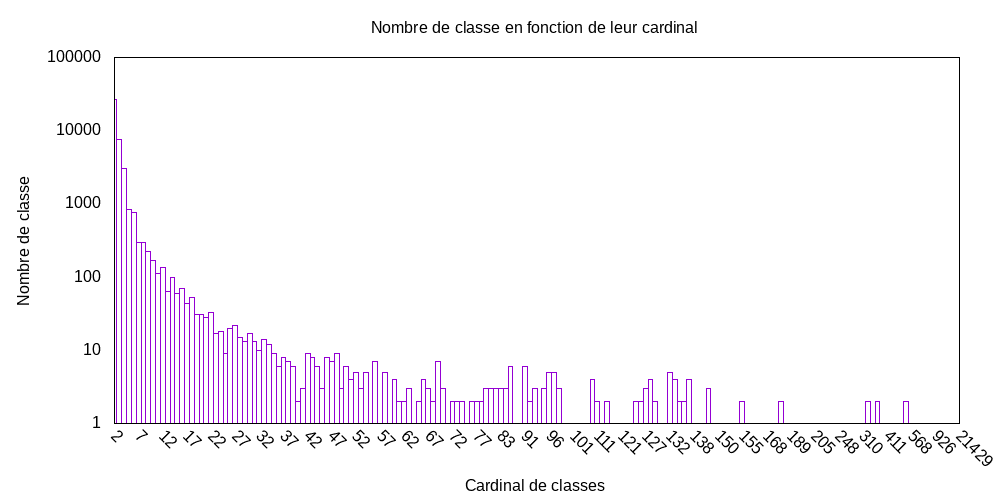
\includegraphics[scale=0.6]{figures/bars.png}
\end{figure}

\paragraph{Aspects qualitatifs}

Les classes comprenant plus de 50 éléments sont majoritairement:
\begin{itemize}
\item Soit des très petites fonctions (des variables globales ou des fonctions constantes). Comme {\Asak} ne prend pas en compte la valeur des littéraux, ces dernières sont toutes regroupées.
\item Soit du code généré par des outils comme \verb|Coq|, \verb|Menhir|, \verb|AWS|...
\end{itemize}

Cependant, certaines classes représentent de véritables possibilités de factorisation. Par exemple, nous trouvons une classe contenant $122$ éléments comprenant toutes les définitions de la (célèbre) fonction \iocaml{Option.map}, que l'on trouve sous pas moins de $32$ noms différents. Cette classe capture aussi les fonctions similaires concernant les types isomorphes au type \iocaml{option}. Par exemple, cette classe contient la fonction \iocaml{map_evar_body} (provenant du module \iocaml{Evd} de \verb|Coq|):

\begin{minted}{OCaml}
let map_evar_body f = function
  | Evar_empty -> Evar_empty
  | Evar_defined d -> Evar_defined (f d)
\end{minted}


\section{Limitations}
\label{sec:limitations}
%!TEX root = root.tex

Nous programmons souvent en utilisant des constructions semblant
similaires mais qui sont belles et bien des constructions sémantiquement
différentes. Cependant {\Asak} est par définition très sensible à la
forme de l'arbre {\LambdaCode} et ce "presque-sucre syntaxique" fait
différer les arbres de codes pourtant très proches. Il en résulte
qu'{\Asak} n'est \emph{pas} adapté à la détection de plagiat. Voici deux illustrations.

\paragraph{L'ordre des définitions}

L'ordre des définitions locales dans une fonction parait anodin mais il influe grandement le calcul d'empreinte puisque celui-ci est effectué récursivement. Il serait alors simple pour quelqu'un désirant fausser les résultats de réorganiser le code afin que sa sémantique reste préservée mais les arbres {\LambdaCode} produit engendrent des empreintes différentes.

\paragraph{L'expansion des définitions}

Nous remplaçons souvent mentalement les variables par leur
définition. Il s'agit cependant d'une opération complexe qui affecte
souvent la sémantique du programme et que le compilateur se risque
rarement à faire. Il en résulte que deux codes ayant exactement la
même sémantique, l'un ayant une multitude de définitions factorisées
et l'autre non engendrent des arbres très différents et donc des empreintes différentes.


\section{Travaux connexes}
\label{sec:related-work}
La comparaison de code est un sujet énormément étudié.  Différentes
analyses détaillées des techniques existantes ont déjà été faites par
Roy et al. \cite{ComparisonAndEvaluation} et Gautam et
al. \cite{variousCodeClone}.  On peut grouper les différentes
approches en quatre grandes familles qui utilisent chacune plus ou
moins la sémantique du langage dans lequel le code est écrit.

\paragraph{Approche textuelle}
Il s'agit ici de comparer directement les chaines de caractères
composant le code, avec le plus souvent un pré-traitement visant à
supprimer les espaces inutiles et les commentaires. Cette approche est
la seule indépendante du langage (à l'exception de la phase de
pré-traitement). Elle a été mise en œuvre dans des outils comme Duploc
\cite{ALanguageIndependent}.

\paragraph{Approche lexicale}
D'autre outils choisissent de travailler sur la séquence de tokens
correspondant au code. Ces outils deviennent donc dépendant d'un
langage mais permettent de résoudre certains problèmes de l'approche
purement textuelle (on est par exemple capable d'identifier deux codes
égaux à $\alpha$-renommage près).  Cette méthode est implémentée dans
des outils comme CC-Finder \cite{ccfinder}, CP-Miner \cite{cpminer} et
DUP \cite{dup}.

\paragraph{Approche syntaxique}
Une autre approche est d'utiliser directement l'arbre de syntaxe
abstrait correspondant au code. Elle est donc dépendante du langage et
permet de résoudre certains problèmes de l'approche lexicale. Cette
méthode a été popularisée avec CloneDr \cite{CloneDetectionUsingAST}
et utilisée plus récemment par Deckard \cite{Deckard}.

\paragraph{Approche sémantique}
Enfin, on peut aussi utiliser les graphes de dépendance
\cite{PdgOrigin} du programme. Ces derniers permettent d'introduire
beaucoup de sémantique dans la détection de clone mais la technique
repose sur la recherche de sous-graphes identiques maximaux, problème
qui est NP-complet. Des approximations en temps polynomial permettent
néanmoins d'obtenir de bons résultats, comme l'a montré Krinke
\cite{PDG}.


\section{Conclusion et travaux futurs}
\label{sec:conclusion}
Dans cet article, nous avons présenté l'approche suivie par~{\Asak} pour
la détection de clones de programmes~{\OCaml} ainsi que des résultats
préliminaires concernant l'application de cet outil à {\LearnOCaml}
et à l'analyse du corpus de paquets {\Opam}.
%
Pour pallier aux limitations que nous avons explicitées, nous allons continuer
à améliorer la prise d'empreintes pour la rendre plus robuste à certaines
transformations syntaxiques locales qui préservent la sémantique.
%
Enfin, en intégrant {\Asak} à un outil comme {\Merlin}, nous allons proposer
au programmeur un outil pour éviter d'introduire de la redondance dans
les programmes~{\OCaml}.

Pour finir, les auteurs remercient la Fondation OCaml et ses sponsors pour
avoir rendu possible le stage de licence d'Alexandre Moine sans lequel
{\Asak} n'aurait pas pu voir le jour.



\bibliographystyle{plain}
\bibliography{publications}

\end{document}
